%%%%%%%%%%%%%%%%%%%%%%%%%%%%%%%%%%%%%%%%%%%%%%%%%%%%%%%%%%%%%%%%%%%%%%%%
\section{Assignment}
\subsection{Overview}
In this lab report we aim to learn and show some
 of the basic functionality of SPENVIS and use this to gain information on and illustrate the plasma environment local to Earth. In the first assignment downloaded a file and looked through it to visually get a feel for the information it was showing. This
 allowed us to use the physical knowledge we had to match real data to our expectations.
 
 
\subsection{Results}

Data was downloaded from \url{http://sidc.be/silso/datafiles} and \url{ftp://ftp.ngdc.noaa.gov/STP/GEOMAGNETIC_DATA/INDICES/KP_AP}, year 2003, and the data format was checked.


\subsection{Discussion}
The data was separated into columns and using the
 key provided in the lab report we were able to identify the flux qualifier, basic information (date) and the sunspot number. This is important as we can check for anomalies or use the format of the data to export and use the data in our own programs as necessary.



%%%%%%%%%%%%%%%%%%%%%%%%%%%%%%%%%%%%%%%%%%%%%%%%%%%%%%%%%%%%%%%%%%%%%%%%
\section{Assignment}
\subsection{Overview}
In this Assignment we modify the settings for the model IRI2001 with the data gathered in the previous task, and re-run the IRI2001 model.
The results are then compared to the default case.
\subsection{Results}

%\begin{figure}[!h]
%	\centering
%	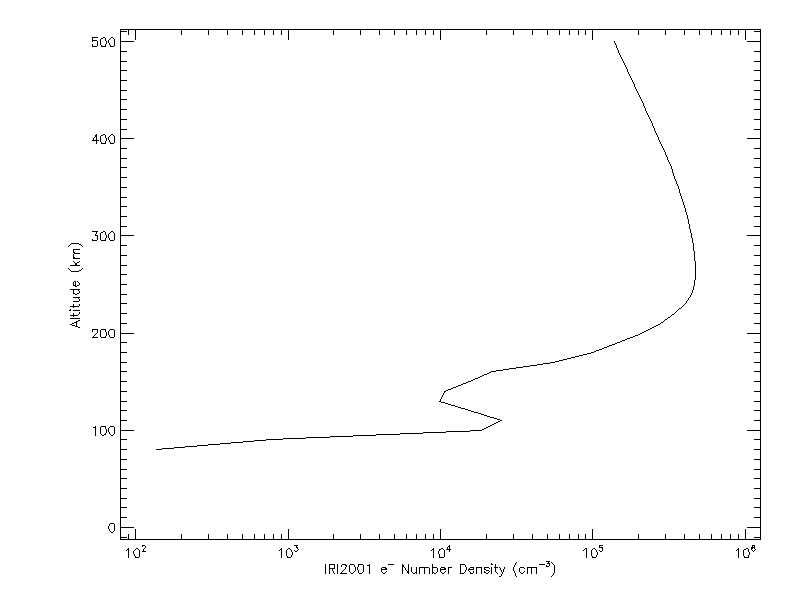
\includegraphics[width=\linewidth]{images/E_number_density_plot1}	
%	\caption{fig:ass2Plot1}
%	\label{fig:ass2Plot1}
%\end{figure}
%\begin{figure}[h]
%	\centering
%	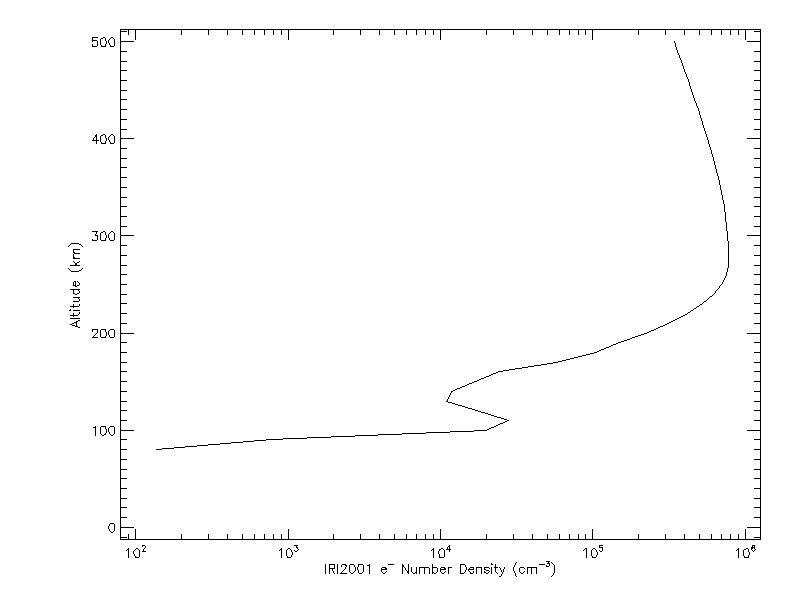
\includegraphics[width=\linewidth]{images/E_number_density_plot2}	
%	\caption{Electron number density Plot New}
%	\label{fig:ass2Plot2}
%\end{figure}


\begin{figure}[!htbp]
  \centering
  \begin{minipage}[b]{0.7\textwidth}
    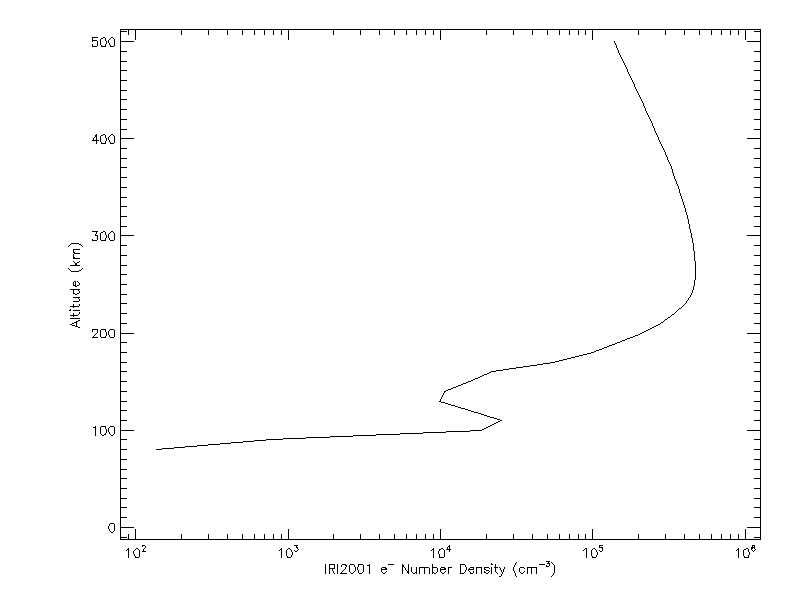
\includegraphics[width=\textwidth]{images/E_number_density_plot1}
    \caption{Electron number density Plot Old}
    \label{fig:ass2Plot1}
  \end{minipage}
  \vfill
  \begin{minipage}[b]{0.7\textwidth}
    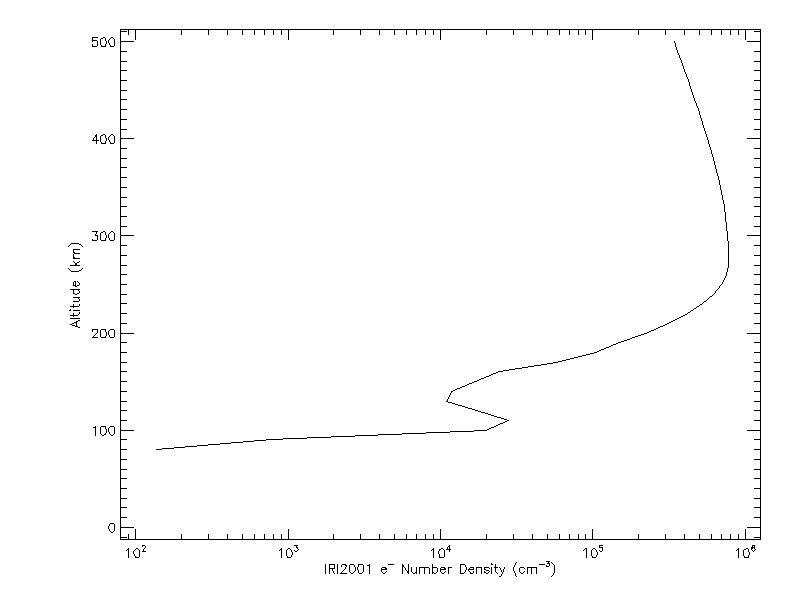
\includegraphics[width=\textwidth]{images/E_number_density_plot2}
    \caption{Electron number density Plot New}
    \label{fig:ass2Plot2}
  \end{minipage}
\end{figure}

\newpage
\subsection{Discussion}
For the default case, the number density is much lower at higher altitudes than it is for the corrected value, for example: at an altitude of approx. 500km the number density is around $10^{5.05}$, whereas for the latter case the number density at 500km is approx. $10^{5.2}$.





%%%%%%%%%%%%%%%%%%%%%%%%%%%%%%%%%%%%%%%%%%%%%%%%%%%%%%%%%%%%%%%%%%%%%%%%
\section{Assignment}
\subsection{Overview}
The model IRI2001 used in Assignment 1 is used again. The year shall stay the same, but other parameters as Day of Year, the daily $F_{10.7}$ and the 12 month average sunspot number are changed.
\subsection{Results}
We used the following values for the parameters to be changed
%\todo{make a table here or something}

\begin{itemize}
	\item year 2003
	\item SD:7.1
	\item average sunspot number 99.3
	\item selected day: 1
\end{itemize}

\begin{figure}[h]
	\centering
	\includegraphics[width=\linewidth]{images/ass3plot1}	
	\caption{Electron number density with standard deviation}
	\label{fig:ass3Plot1}
\end{figure}

The sunspot number parameter has almost no effect at lower altitudes, however at approx. 250km the electron number density starts to vary. The lower the sunspot number the lower the electron number density at each respective altitude above 250km.
%\todo{insert plot here km/e-}

2. The electron number density varies on a diurnal basis, but only very minutely. 

3. Comparing Winter and Summer (day 1 and day 181), the electron number density varies on a larger scale.
\subsection{Discussion}
These results have wider implications for satellites
 in space. As the sunspot number varies the number density of electrons varies. This means that there is a changing electron flux as the spacecraft travels through space and the maxima and minima need to be accounted for in any physical specifications for the
 electronics and material property analysis. There is also variation in both day and season. This also needs to be accounted for in estimations of maximum and minimum flux to ensure that a spacecraft does not unexpectedly fail due to the varying flux.


%%%%%%%%%%%%%%%%%%%%%%%%%%%%%%%%%%%%%%%%%%%%%%%%%%%%%%%%%%%%%%%%%%%%%%%%
\section{Assignment}
\subsection{Overview}
In this assignment we will study the ionosphere and
 take into account the limitations and strengths of the IRI2001 model. By doing this we will gain insight into how models are used and ways we can modify them to account for the limiting factors.
\subsection{Results}
Since the given latitude and longitude are located in the auroral region, and 2003 was close to a maximum of the sun's 11-year cycle, the IRI2001 Model is not suitable as this is not magnetically-quite region.
\subsection{Discussion}
This assignment showed us how the models are only
 suitable for certain conditions and real situations do not always meet the conditions required for the model. This may render the model only partially applicable or completely useless. By looking at the conditions in space we can decide how appropriate the
 models are and explain any failures in the model. This will allow us to improve upon the model in later iterations of the model and this allows us to make better predictions of the space environment for the future.


%%%%%%%%%%%%%%%%%%%%%%%%%%%%%%%%%%%%%%%%%%%%%%%%%%%%%%%%%%%%%%%%%%%%%%%%
\section{Assignment}

\subsection{Overview}
For this assignment, the year 2012 was utilized  in order to determine the ionospheric layers. The corresponding day of the year, Daily $F_{10.7}$, and Sunspot Number were 270, 139.9, and 84.5, respectively. The coordinating grid was kept the same as previous assignments. The figure below diplays the number density of various particles and ions as the altitude is varied. 
\newpage
\subsection{Results}

	\begin{figure}[!h]
		\centering
		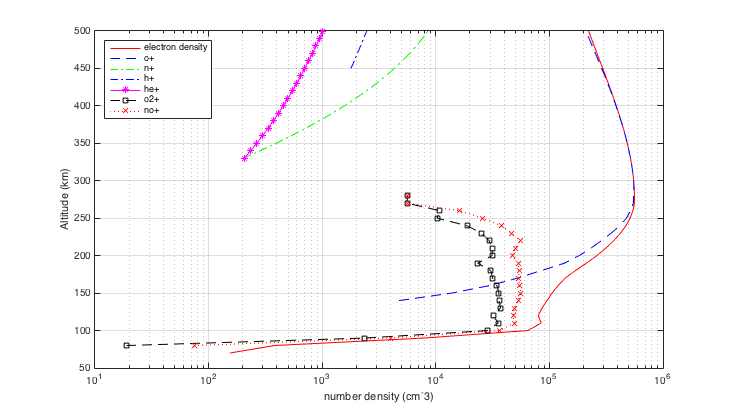
\includegraphics[width=\linewidth]{images/ass5_properties_plot}
		\caption{Altitude vs. Particle Number Density ($cm^{-3}$)}
	\end{figure}
The results are also looked at more closely in the
 Discussion section.
\subsection{Discussion}
		Based on the densities shown in the particle density graph, it can be seen that D-layer exists between ~50-100 km. The presence of low amounts of NO ions corroborates the aforementioned statement as only a high-wavelength spectral line would be able to penetrate to this level and ionize the heavy ions. 
		\par
		The E-layer is somewhere between ~95-150 km. This layer consists of high amounts of $0_2^+$ and $N_2^+$ ions which are produced when x-rays and ultraviolet rays dissociate $O_2$ and $N_2$ molecules.
		\par
		The F layers is divided into the F1 and F2 layers. The F1 layer exists from between ~150-220 km. This can be determined by seeing the number density of electrons and $O^+$. Electron density is somewhere between $5e5$ to $5e6$ and $O^+$ density is higher due to the lighter particle floating to the higher regions. The F2 layer is between ~200-500 km. The lighter ions such as $He_+, N^+, and H^+$  exist in this layer due to their light weight.
		\par
		The Chapman layer differs from IRI model in displaying the number densities of particles especially in the F2 layer. These differences exist because the Chapman layer takes into account some parameters that the IRI model does not and vice versa. For example, the Chapman layer takes into account the Sun's zenith angle. In addition, the chapman layer method assumes that the radiation from sun is monochromatic, the atmosphere consists of only one gas, etc. These assumptions allow the chapman layer to create a "better density profile especially for the topside ionosphere (Jin)".


% References

% http://center.shao.ac.cn/geodesy/publications/Jin_2007EPS.pdf
% http://nova.stanford.edu/~vlf/IHY_Test/Tutorials/TheIonosphere/IonosphericMorphology.pdf



%\subsection{Overview}
%\subsection{Results}
%\todo{todo}
%D-Layer below 90
%
%E 90-130
%
%F1-130
%\begin{figure}[h]
%	\centering
%	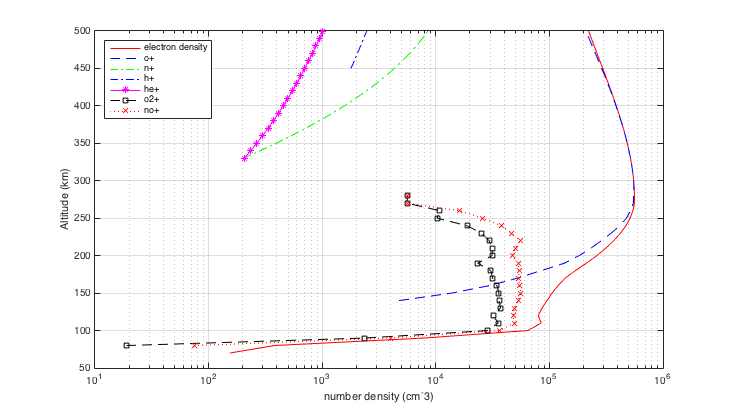
\includegraphics[width=\linewidth]{images/ass5_properties_plot}	
%	\caption{bla}
%	\label{fig:ass5Plot}
%\end{figure}
%
%
%\subsection{Discussion}

